\newpage
%\section{Problem Setup}
\chapter{Model formulation}
\label{Chapter_Problem_setup}
%Describe the box task, both versions. 
The box task is an information sampling task that is used to assess a 'jumping to conclusions' (JTC) bias \citep{balzan2017}. In the box task used in this report the participants are shown a grid of twelve boxes, and each time a box is opened, one out of two colours, for example blue or red, is displayed. The participants are told that one of the colours is always in majority, and that their task is to find out which one. We are using two different versions of the box task. In the first one the participant can open as many of the twelve boxes as they want before deciding which of the two colours that is in majority. We call this the unlimited version. In the second one, which we call the limited version, the participants are told that the test will terminate at one point when a random box is opened. If the participant have not decided what the majority colour is when the test terminates, this counts as a failed trial. 

We have data from 76 participants that have done multiple trials of both versions of the box task. The experiment where the data was collected was carried out by Professor Gerit Pfuhl and Doctoral Research Fellow Kristoffer Klevjer at UiT The Arctic University of Norway in February 2020. The participants were recruited from an undergraduate psychology course. They did a practice limited trial first that terminated after three boxes where opened, such that if they tried to open a fourth box, the test terminated, and they were not able to make a decision. That trial is not analyzed here. Following the practice trial where three unlimited trials. The participants could in these trials open as many of the twelve boxes as they wanted before deciding on what they think is the dominant colour. Lastly, there where six limited trials. Three of them terminated after six boxes had been opened and the other three terminated after nine boxes had been opened. These are the trials we analyze, thus we analyze trial 2 to 10. We have data for how many boxes each participant opened before they either chose what they believed was the majority colour, or the test terminated, we call this 'draws to decision'. In addition to this we have information about the choice they made for what the majority colour was, or weather the test terminated before they were able to choose. To compensate for possible biases towards one colour, the two colours where changed for each new trial. They could for example be green and pink in the first trial and blue and yellow in the second trial. For simplicity, we are referring to these colour as blue and red for all trials in this report.

For each trial there is a fixed sequence of boxes. The participants are only able to choose whether to open the next box or not, not which box that opens. Thus, we know how many of the boxes that were blue and how many that were red for each step in the trials. In Figure \ref{fig:trial2_order}, we see the order the boxes are opened in in trial 2, which is an unlimited trial. In Figure \ref{fig:histogram_trial2}, the draws to decisions for all participants are shown in a histogram. Here, the number of boxes that are opened when the participant chooses what he thinks is the majority colour is on the horizontal axis. On the vertical axis are the number of participants that has chosen on that particular box. We see that many participants have chosen majority colour after three boxes are opened. All of these three boxes are red, thus, there is a high probability that red is the dominant colour. 
As the participants are told that one of the colours always is in majority, we can be completely sure if six of the opened boxes are red, that red is the dominant colour. This is because there cannot be six of each box if one of them is in majority. When seven boxes are opened in trial 2, six of them are red, and we know then that red is the dominant colour. Seven participants have chosen colour after seven boxes are opened. (hvor mye skal jeg skrive om dette?)
\begin{figure}
    \centering
    \scalebox{0.8}{\begin{tikzpicture}[node distance = 1.2cm]
    \node (1) [red_trial]{}; 
    \node (2)[red_trial, right of=1]{};
    \node (3)[red_trial, right of=2]{};
    \node (4)[blue_trial, right of=3]{};
    \node (5)[red_trial, right of=4]{};
    \node (6)[red_trial, right of=5]{};
    \node (7)[red_trial, right of=6]{};
    \node (8)[red_trial, right of=7]{};
    \node (9)[blue_trial, right of=8]{};
    \node (10)[red_trial, right of=9]{};
    \node (11)[blue_trial, right of=10]{};
    \node (2)[red_trial, right of=11]{};
\end{tikzpicture}}
    %\includegraphics{}
    \caption[Order of boxes in trial 2]{The order of the boxes in trial 2. This is an unlimited trial.}
    \label{fig:trial2_order}
\end{figure}


\begin{figure}
    \centering
    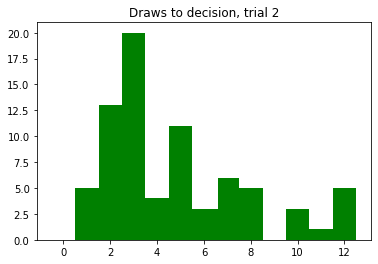
\includegraphics[scale=0.6]{pictures/dtd2_histogram.png}
    \caption[Draws to decisions in trial 2]{Histogram of the draws to decisions for all participants in trial 2. 
    har forandret på denne figurern, husk å bytte til riktig!!}
    \label{fig:histogram_trial2}
\end{figure}


In trial 3, which also is an unlimited trial, it takes more boxes to be completely sure what the majority colour is. As shown in Figure \ref{fig:trial3_order}, there are six blue boxes when ten of the boxes are opened. We see in Figure \ref{fig:histogram_trial3} that the participants in general open more boxes before choosing the majority colour in this trial than in trial 2. 

\begin{figure}
    \centering
    \scalebox{0.8}{\begin{tikzpicture}[node distance = 1.2cm]
    \node (1)[blue_trial]{}; 
    \node (2)[red_trial, right of=1]{};
    \node (3)[blue_trial, right of=2]{};
    \node (4)[red_trial, right of=3]{};
    \node (5)[blue_trial, right of=4]{};
    \node (6)[blue_trial, right of=5]{};
    \node (7)[red_trial, right of=6]{};
    \node (8)[blue_trial, right of=7]{};
    \node (9)[red_trial, right of=8]{};
    \node (10)[blue_trial, right of=9]{};
    \node (11)[red_trial, right of=10]{};
    \node (2)[blue_trial, right of=11]{};
\end{tikzpicture}}
    %\includegraphics{}
    \caption[Order of boxes in trial 3]{The order of the boxes in trial 3. This is an unlimited trial.}
    \label{fig:trial3_order}
\end{figure}

\begin{figure}
    \centering
    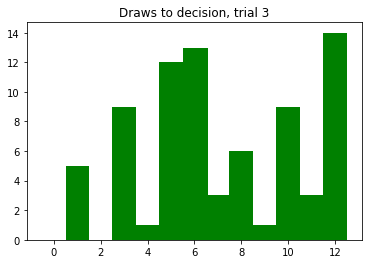
\includegraphics[scale=0.6]{pictures/dtd3_histogram.png}
    \caption[Draws to decisions in trial 3]{Histogram of the draws to decisions for all participants in trial 3. 
    har forandret på denne figurern, husk å bytte til riktig!!}
    \label{fig:histogram_trial3}
\end{figure}

Both trial 5 and 8 are limited trials that terminates after nine boxes are opened. The order of the boxes in trial 5 is shown in Figure \ref{fig:trial5_order}. When seven boxes are opened, six of them are blue, and we can therefore conclude when seven boxes are opened that blue is the majority colour. We see in Figure \ref{fig:histogram_trial5} that many participants chooses majority colour after three boxes are opened, when there are only blue boxes. In trial 8 there are never two boxes of the same colour following each other, as shown in Figure \ref{fig:trial8_order}. There are never six of one of the colours, meaning that we never can be completely sure which one is the majority colour. This is reflected in the draws to decision for the participants, as shown in Figure \ref{fig:histogram_trial8}. We see that the test terminates for many of the participants before they are able to choose what they think is the majority colour. 

\begin{figure}
    \centering
    \scalebox{0.8}{\begin{tikzpicture}[node distance = 1.2cm]
    \node (1)[blue_trial]{}; 
    \node (2)[blue_trial, right of=1]{};
    \node (3)[blue_trial, right of=2]{};
    \node (4)[red_trial, right of=3]{};
    \node (5)[blue_trial, right of=4]{};
    \node (6)[blue_trial, right of=5]{};
    \node (7)[blue_trial, right of=6]{};
    \node (8)[blue_trial, right of=7]{};
    \node (9)[red_trial, right of=8]{};
\end{tikzpicture}}
    \caption[Order of boxes in trial 5]{The order of the boxes in trial 5. This is a limited trial that terminates after nine boxes are opened.}
    \label{fig:trial5_order}
\end{figure}
\begin{figure}
    \centering
    \scalebox{0.8}{\begin{tikzpicture}[node distance = 1.2cm]
    \node (1)[blue_trial]{}; 
    \node (2)[red_trial, right of=1]{};
    \node (3)[blue_trial, right of=2]{};
    \node (4)[red_trial, right of=3]{};
    \node (5)[blue_trial, right of=4]{};
    \node (6)[red_trial, right of=5]{};
    \node (7)[blue_trial, right of=6]{};
    \node (8)[red_trial, right of=7]{};
    \node (9)[blue_trial, right of=8]{};
\end{tikzpicture}}
    \caption[Order of boxes in trial 8]{The order of the boxes in trial 8. This is a limited trial that terminates after nine boxes are opened.}
    \label{fig:trial8_order}
\end{figure}
\begin{figure}
    \centering
    \begin{minipage}{0.45\textwidth} 
        \centering
        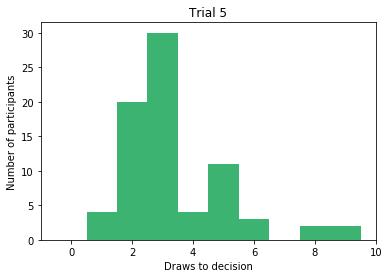
\includegraphics[scale=0.4]{pictures/dtd5_histogram.png}
        \caption[Draws to decisions in trial 5]{write caption}
        \label{fig:histogram_trial5}
    \end{minipage}\hfill
    \begin{minipage}{0.45\textwidth} 
        \centering
        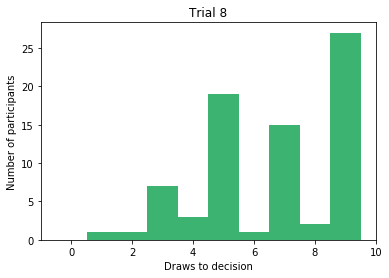
\includegraphics[scale=0.4]{pictures/dtd8_histogram.png}
        \caption[Draws to decisions in trial 8]{Write caption}
        \label{fig:histogram_trial8}
    \end{minipage}
\end{figure}

(burde jeg si et sted at resten av trialsene finnes i appendix? hvis jeg skal ha det med da?)

In this chapter, we formulate a model for how decisions are made in the box task, and we want to find parameter estimates such that we can adjust/fit the model to each person. We also find a so-called Ideal Observer solution of the box task. An Ideal Observer would always make optimal decisions \citep{idealObs}. Thus, an Ideal Observer solution is close to an optimal solution of the box task. 



\section{Modelling Framework}
Before we start with the formulation of the model, we will introduce some notation and present some assumptions. 

\label{section_notation}
Let $X_i$ be the colour of the $i$-th opened box. If the box is blue, $X_i$ is 0 and if the box is red, $X_i$ is one. Thus,
\begin{equation*}
    X_i = \begin{cases}
    0,& \quad \text{if box } i \text{ is blue,}\\
    1,& \quad \text{if box } i \text{ is red.}
    \end{cases}
\end{equation*}
We assume that each $X_i$ has a Bernoulli distribution with success probability $\theta$, such that
\begin{equation*}
    X_i \sim \text{Bernoulli}(\theta).
\end{equation*}
We define a vector, $X_{1:i}$, that, when $i$ boxes are opened,
contains the colours of all these $i$ boxes, such that $X_{1:i} = (X_1,X_2,...,X_{i})$. In the same way, when we have observed data, $(X_1=x_1,X_2=x_2,...,X_i=x_i)$, we denote this as $x_{1:i}$.
%Maybe denote $\textbf{X} = (X_1,X_2,...,X_{12})$ or $\textbf{X}_{12} = (X_1,X_2,...,X_{12})$ and $x_{1:i} = (X_1,X_2,...,X_{i})$?

Additionally, let $U_i$ be the number of the first $i$ opened boxes that are red. Thus, $U_i$ is a stochastic variable defined as
\begin{equation*}
    U_i = \sum_{j=1}^{i} X_j. 
\end{equation*}
The sum of Bernoulli distributed variables is binomial distributed \citep{statinf}. Thus, $U_i$ is binomially distributed with parameters $i$ and $\theta$. We define another stochastic variable, $V_i$, that is the number of red boxes that are not opened when $i$ boxes are opened. Thus, $V_i$ is the number of red boxes out of the $12-i$ boxes that are not opened, which yields,
\begin{equation*}
    V_i = \sum_{j=i+1}^{12} X_j.
\end{equation*}
This variable is also binomially distributed, but with parameters $12-i$ and $\theta$. Thus,
\begin{equation}
\label{U_V_binomal_distri}
    \begin{aligned}
        U_i &\sim \text{Binomial}(i,\theta)\\
        V_i &\sim \text{Binomial}(12-i,\theta).
    \end{aligned}
\end{equation}
%\begin{subequations}
%\begin{equation}
%\label{U_binomail_distr}
%    U_i \sim \text{Binomial}(i,\theta)
%\end{equation}
%\begin{equation}
%\label{V_binomial_distr}
%    V_i \sim \text{Binomial}(12-i,\theta).
%\end{equation}
%\end{subequations}
Then, we have that 
\begin{equation}
\label{ui_prob_mass}
    P(U_i=u_i|\Theta=\theta) = \binom{12}{u_i} \theta^{u_i}(1-\theta)^{12-u_i},
\end{equation}
and
\begin{equation}
\label{vi_prob_mass}
    P(V_i=v_i|\Theta=\theta) = \binom{12-i}{v_i} \theta^{v_i}(1-\theta)^{12-i-v_i},
\end{equation}

Just as in Chapter \ref{theory_bayesian_modelling}, we let $\theta$ have a beta prior with parameters $\gamma$ and $\kappa$. (burde jeg skrive om hvorfor her? eller holder det at jeg sier at de er konjugert i 2.4?)
Thus, 
\begin{equation}
\label{beta_prior_theta}
    \theta \sim \text{Beta}(\gamma,\kappa).
\end{equation}
The prior distribution of $\theta$ is then
\begin{equation}
\label{beta_density_func}
    f(\theta) = \frac{1}{\text{B}(\gamma,\kappa)}\theta^{\gamma-1}(1-\theta)^{\kappa-1}.
\end{equation}

Figure \ref{fig:pdf_beta_distr} shows the probability density function of the beta distribution for different values of $\gamma$ and $\kappa$. The pink line represents the situation where $\gamma=\kappa=1$. This is the same as a uniform prior for $\theta$. That means that the probability of $\theta$ being anywhere on the interval between 0 and 1, is constant. As the participants are told that one of the colours will be in majority, but get no information about which one, this might be a suitable prior.
However, one might argue that our prior beliefs resembles more the purple or orange lines as we know that one of the colours will definitively be in majority, thus it is not really reasonable to assume that $\theta$ is 0.5. For this reason we also exclude all priors that have $\gamma$ and $\kappa$ larger than 1, which is the situation for the black and grey lines. (Litt usikker på om dette skal være med her, eller lenger nede når jeg snakker om resultatene?)

\begin{figure}
    \centering
    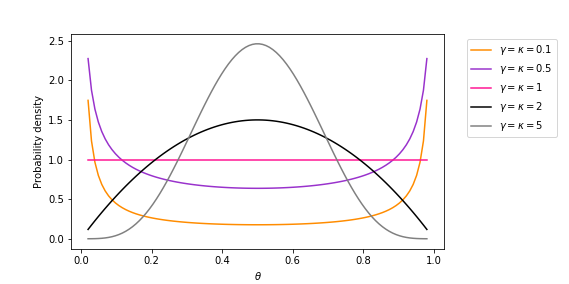
\includegraphics[scale=0.5]{pictures/beta_pdf.png}
    \caption{Caption}
    \label{fig:pdf_beta_distr}
\end{figure}


Of all the 12 boxes, $U_i+V_i$ is the total number of red boxes.
Consequently, if $U_i+V_i$ is bigger than 6, it is a red majority in the box task, and if it is smaller than 6, the true majority colour is blue. We denote this true majority colour as $Z$, such that
\begin{equation}
\label{def_of_Z_2}
    Z = I(U_i+V_i>6).
\end{equation}
This is the same as defining $Z$ as in \eqref{def_of_Z}, as $U_i+V_i = \sum_{j=1}^{12}X_j$, and the order that the boxes are opened in does not affect the majority. Then, as in \eqref{Z_true_majority}, $Z$ is 0 if the true majority colour is blue and 1 if the true majority colour is red. 


%Each time a box is opened, we have three choices. The first is to choose that blue is the majority colour, the second that red is and the third is to open another box. Let $\delta_{i+1}$ denote the different choices when $i$ boxes are opened. If $\delta_{i+1}=0$, we have chosen that blue is the majority colour, $\delta_{i+1}=1$ shows that red is chosen as the majority and $\delta_{i+1}=2$ represents the choice of opening the next box, which is box $i+1$. Moreover, let $\delta_{(i+2):12}$ be the choices made after box $i+1$ is opened. 

Each time a box is opened, the participants have three choices. The first is to choose that blue is the dominant colour, the second that red is, and the third is to choose to open another box. We denote these decisions as $\delta_i$, where $i$ is the number of boxes that are opened. If $\delta_i = 0$, the participant chooses that blue is the more prominent colour, thus that there are in total, of all twelve boxes, more blue boxes than red. Moreover, $\delta_i=1$ means that the participant has chosen that red is the dominant colour, and $\delta_i=2$ represents the situation where the participant chooses to open the next box. Thus,
\begin{equation}
\label{def_of_delta}
    \delta_i =
    \begin{cases}
        0,& \quad \text{if blue is chosen as majority colour,}\\
        1,& \quad \text{if red is chosen as majority colour,}\\
        2,& \quad \text{if the participant chooses to open the next box.}
    \end{cases}
\end{equation}
%We denote the choices that are made from when $i$ boxes are opened to the last choice is made as $\delta_{i:12}$. Something about not making decisions after majority colour is chosen, such that for example $\delta_{12}$ might not exist. dette trgner jeg ikke hvis jeg isf bruker IO(\textbf{x}$_i,\delta_{i+1}$).

We can define loss functions for each of these decisions. These loss functions depend on the true majority colour, $Z$, and the decision that is made, $\delta_i$. Similarly to Chapter \ref{theory_loss_functions}, we denote the loss function when $i$ boxes are opened as $L_i[Z,\delta_i]$. In our case, we have that 
\begin{equation*}
    \Omega_Z = \{0,1\}
\end{equation*}
and 
\begin{equation*}
    \Omega_{\delta_i}=\{0,1,2\}.
\end{equation*}
%$\Omega_Z = \{0,1\}$ and $\Omega_{\delta_i}=\{0,1,2\}$.


If we take the expectation of this loss function, we get the expected loss for each of these decisions when $i$ boxes are opened, which we denote $\EE^i_{\delta_i}(\theta)$, as it depends on some parameters $\theta$. This expected loss also depends on the colours of the $i$ boxes that already are opened, $x_{1:i}$.

In the limited version of the box task, the participants are told that the test will terminate when a random box is opened. Thus, we need a random variable that represents how many boxes that are open when the test terminates. We call this variable $T$. If $T=3$, then the participant has opened three boxes and wants to open the fourth. Instead of seeing the colour of the fourth box, the test terminates. The information given to the participants regarding this is that the test will terminate when a random box is opened. We assume that the first box always can be opened, but that the probabilities that the test terminates at the subsequent boxes are the same. When 12 boxes are opened, there are no more boxes to open, thus, no more chances for the test to terminate. Thus, $T$ is uniformly distributed with values $(1,2,3,4,5,6,7,8,9,10,11)$, 
\begin{equation}
\label{T_uniform}
    T \sim \text{Uniform}({1,2,3,4,5,6,7,8,9,10,11}).
\end{equation}

Now we have all the notation needed to define the model for how the participants make decisions. 

\section{The Model for Decisions/something else}
Having the notation for the expected losses and decisions, we can define the probability mass function for the decisions using a softmax function similar to the one in \eqref{softmax_in_theory}. 

For each participants we have observed decisions, $\boldsymbol{\delta}=(\delta_1,\delta_2,...,\delta_n)$, where $\delta_j \in \{0,1,2 \}$ as in \eqref{def_of_delta}, and $n$ is the total amount of decisions we have for each participant. Thus, $j\in \{1,2,...,n \}$. As the participants have opened a different amount of boxes each time, $n$ varies form participant to participant. Recall that $i$ is the number of boxes that are opened, and that $i$ is reset for each new trial. Thus, the probability mass function for the decisions can be expressed as (er ikke denne egentlig $f(\delta_j|\theta,\eta,x_{1:i})$ ???)
\begin{equation}
\label{softmax_theta}
    f(\delta_{j}|\theta,\eta) = \frac{\text{exp}(- \eta \EE^i_{\delta_{j}}(\theta))}{\sum_{d=0}^{2} \text{exp}(-\eta \EE^i_{d}(\theta))},
\end{equation}
where $\eta$ is some parameter. This can be interpreted as a measure of how far the choices the participants make are away from the decision with the least expected loss. If $\eta$ is infinity, they always make the decision with the lowest expected loss, and if $\eta$ is zero, they choose arbitrarily. A negative value of $\eta$ indicates that the participant tends to choose the decisions with the highest expected losses.


When we have this model, we can find estimates of the parameters $\theta$ and $\eta$ for each participant such that the model is adapted to each one of the participants. This is done by finding the maximum likelihood estimates (MLEs) as described in Chapter \ref{section_theory_mle}. 
We can also find confidence intervals tied to each of the parameters for all of the participants using the bootstrap as described in Chapter \ref{section_theory_bootstrap}. This will be done in the subsequent sections, but firstly we find an Ideal Observer solution of the box task, and find expressions for the loss functions and expected losses. 


\section{An Ideal Observer Solution of the Box Task}
\sectionmark{An Ideal Observer Solution}
We now want to find an Ideal Observer solution of the box task. As stated above, an Ideal Observer acts like a participant that always makes optimal decisions. In the case of the box task, the optimal decision for each opened box is the decision that gives the least expected loss. If one makes the decision with the lowest expected loss each time a box is opened, the total solution is the Ideal Observer solution. Thus, we need to find these expected losses. 

Recall that when $i$ boxes are opened, the participants has three choices as stated in \eqref{def_of_delta}. We want to find expected losses for all of these three choices, in both the unlimited and limited versions of the box task. As the expected losses are the expectations of loss functions, we firstly need to define some loss functions. 



\subsection{Loss Functions in the Unlimited Case}
Starting with the unlimited case, we find loss functions for each of the three choices we have when $i$ boxes are opened. If the participant chooses blue as the majority colour, when $\delta_i=0$, we say that the loss is 0 if blue actually is the true majority colour and 1 if it is not. Thus, this can be expressed as an indicator function as in \eqref{loss_func_indicator}. Recall that the true majority colour is denoted $Z$. Then, we can express the loss of choosing blue as the majority colour when $i$ boxes are opened as
\begin{equation}
\label{loss_func_blue}
    L_i[Z,\delta_i=0] = I(Z \neq \delta_i) = I(Z\neq0) = I(Z=1).
\end{equation}

We define the loss function for when the participant chooses that red is the majority colour, when $\delta_i=1$, similarly to \eqref{loss_func_blue}. This time the loss is 0 if the true majority colour is red and 1 if the blue is the true majority colour. Thus,
\begin{equation}
\label{loss_func_red}
    L_i[Z,\delta_i=1] = I(Z\neq\delta_i) = I(Z\neq1)=I(Z=0).
\end{equation}
Putting these two loss functions together, we get that the loss when the participant chooses what the majority colour is, when $\delta_i \neq 2$, is 
\begin{equation}
\label{loss_0_1_unlim}
    L_i[Z,\delta_i \neq 2] = I(Z \neq \delta_i). 
\end{equation}

We imagine that some participants have some small penalty or loss of opening another box. This might be because it is tiresome for them to sit through a whole trial and they want to finish fast, or that they get some kind of inner reward or feeling of victory when they finish early. This is represented by a parameter, $\alpha$. (burde jeg egntlig beskrive hva $\alpha$ er i Modelling Assumptions kapittelet?)
The loss function for the choice of opening the next box depends on the successive losses. As we do not know the choices that will be done later, we do not know what these losses are either. However, we can model these choices as the choices that an Ideal Observer would make. These choices depend on the colour of the next box, $X_{i+1}$ and the colours of the boxes that already are opened, $x_{1:i}$. We denote these choices as $IO(x_{1:i},X_{i+1})$, where $X_{i+1} \in \{0,1\}$.
%The loss function for opening the next box depends on the parameter $\alpha$. Recall that this is a small loss, potentially zero, for opening a box. It also depends on the loss after the next box is opened. 
We define the loss for the decision to open the next box as $\alpha$ plus the loss in the next step. Thus, 
\begin{equation}
\label{loss_2_unlim}
    L_i[Z,\delta_i=2] = \alpha + L_{i+1}[Z,IO(x_{1:i},X_{i+1})],
\end{equation}
where $L_{i+1}[Z,IO(x_{1:i},X_{i+1})]$ is the loss when the next box is opened. 


Putting \eqref{loss_0_1_unlim} and \eqref{loss_2_unlim} together, we get that the total loss function in the unlimited case can be expressed as
\begin{equation*}
%\label{tot_loss_unlim}
    \begin{aligned}
       L_i[Z,\delta_{i}] 
       = I(Z \neq \delta_i)I(\delta_i\neq2)
       + \big(\alpha + L_{i+1}[Z,IO(x_{1:i},X_{i+1})] \big) I(\delta_i=2).
    \end{aligned}
\end{equation*}

Having the loss functions for the unlimited case, we proceed with finding the loss functions for the limited trials of the box task. 


\subsection{Loss Functions in the Limited Case}
The loss functions in the limited case are highly comparable to the ones in the unlimited case. Recall that in a limited trial, the participants might be stopped when a random box is opened, and that this counts as a failed trial. 

Firstly, we have a look at the loss function for choosing blue as the majority colour. We see that in the unlimited case, this is not dependent on any of the boxes that are not opened. When $i$ boxes are opened in a limited trial, and the participant chooses that blue is the majority colour, this is, as in the unlimited trial, not affected by the colours of the unopened boxes. If $i$ boxes are opened and one chooses what the majority colour is here, we know that the test will not terminate, as the participant will not open more boxes. Thus, we can put the loss function for choosing blue as the majority colour in a limited trial as the same as the loss function for choosing blue in an unlimited trial. Thus the loss function is as in \eqref{loss_func_blue}.

The same argument holds for the loss function for choosing red as the majority colour in a limited trial. Thus, that loss function is the same as in \eqref{loss_func_red}.

For the choice of opening the next box, we have to consider that the test might terminate. 
We define a parameter, $\beta$, that only appears in the loss function for opening the next box in limited trials. 
We let it be the loss the participant gets/feels when the test terminates before he or she is able to choose what the majority colour is.
%Recall that $\beta$ is the loss when the test terminates and that $T$ is the number of boxes that already are opened when the test terminates. 
Recall that $T$ is the number of boxes that already are opened when the test terminates, and that it is uniformly distributed as in \eqref{T_uniform}. The loss when the test does not terminate will be the loss for when the next box is open, in the same way as for the unlimited trials. We can include the event of the test terminating as an indicator function, where an indicator function is as seen in \eqref{loss_func_indicator}. Thus, the loss function for opening the next box in an unlimited trial is the loss you get when the next box is opened plus $\alpha$, times an indicator function that is one if the test does not terminate. I addition to this we have the loss for when the test terminates, $\beta$, times an indicator for that the test terminates. Hence,
\begin{equation}
\label{loss_func_2_limited}
    \begin{aligned}
        L_i[Z,\delta_i=2] = \big( \alpha + L_i[Z,IO(x_{1:i},X_{i+1})] \big) \: I(T\neq i) + \beta \: I(T=i),
    \end{aligned}
\end{equation}
where $IO(x_{1:i},X_{i+1})$ are the choices that an Ideal Observer would do in the next steps. 

Now that we have all the loss functions, we can proceed with finding the expected losses. 

\subsection{Expected Losses}
\label{section:exp_losses}
When we find the expected losses we take the expectation of the loss functions as is done in \eqref{expectation_of_loss_func_general}. Recall that taking the expectation of an indicator function gives the probability of the event, and that $x_{1:i}$ is a vector containing the colours of the $i$ opened boxes.

As stated in Chapter \ref{section_notation}, the expected losses when $i$ boxes are opened, are denoted $\EE_{\delta_i}^i(\theta)$, with $\delta_i \in (0,1,2)$.
We start with the expected loss for choosing blue as the majority colour, $\EE^i_0(\theta)$. This is the same for both the unlimited and limited trials as the loss functions, stated in \eqref{loss_func_blue}, are identical. 
We condition on the colours of the opened boxes, as the true majority colour, $Z$, depends on the colours of all the twelve boxes. Thus,
\begin{equation}
\label{exp_loss_blue}
    \begin{aligned}
        \EE^i_{0}(\theta) = &E\big[ L_i[Z,\delta_i=0] \big |x_{1:i} ]\\
        = & E \big[ I(Z=1) \big|x_{1:i}]\\
        = & P(Z=1|x_{1:i}).
    \end{aligned}
\end{equation}
We see that the expected loss of choosing blue as the majority colour is equal to the probability that red is the majority colour given the colours of the opened boxes, for both the unlimited and limited versions. The only thing that this expected loss depends on are the colours of the first $i$ boxes, $x_{1:i}$. Vil det si at $\theta = \emptyset$, eller at $\theta = x_{1:i}$.
%\begin{equation*}
%    \theta = x_{1:i}.
%\end{equation*}

We find the expected loss of choosing red as the majority colour when $i$ boxes are opened, $\EE^i_{1}(\theta)$, similarly to \eqref{exp_loss_blue}. Again, conditioning on $x_{1:i}$, we get
\begin{equation}
\label{exp_loss_red}
    \begin{aligned}
        \EE^i_{1}(\theta) 
        = &E\big[ L_i[Z,\delta_i=1] \big |x_{1:i} ]\\
        = & E \big[ I(Z=0) \big|x_{1:i}]\\
        = & P(Z=0|x_{1:i}).
    \end{aligned}
\end{equation}
The expected loss for choosing red as the majority colour is then the probability that blue is the majority colour, conditioned on $x_{1:i}$, for both the unlimited and the limited case. As above, we see that  $\theta=\emptyset$ eller $\theta = x_{1:i}$.

When we find the expected losses for opening the next box, we have to distinguish between the unlimited and limited cases. Staring with the unlimited case, we continue in the same way as for choosing blue or red as the majority colour, by taking the expectation of the loss function and conditioning on the colours of the $i$ opened boxes. Recall that $IO(x_{1:i},X_{i+1})$ are the choices that an Ideal Observer would do in the next steps. We then get that
\begin{equation*}
    \begin{aligned}
        \EE^i_{2}(\theta) 
        =& E \big[ \alpha + L_i[Z,IO(x_{1:i},X_{i+1})] |x_{1:i}\big].
    \end{aligned}
\end{equation*}
Taking the expectation of a constant gives the constant, thus $E[\alpha|x_{1:i}]=\alpha$, as $\alpha$ is not dependent on the colours of the boxes. Then,
\begin{equation}
\label{exp_loss_unlim_2_unfinished}
    \begin{aligned}
        \EE^i_{2}(\theta) 
        =& \alpha + E \big[L_i[Z,IO(x_{1:i},X_{i+1})] |x_{1:i}\big].
    \end{aligned}
\end{equation}
We see that $E \big[L_i[Z,IO(x_{1:i},X_{i+1})] |x_{1:i}\big]$ is the expected loss in the next step, and it depends on the colour of the box that opens, $X_{i+1}$. We find this expectation using the law of total expectation as in \eqref{law_tot_exp_func}. Then,
\begin{equation}
\label{exp_loss_next_unlim}
    \begin{aligned}
        E \big[L_i&[Z,IO(x_{1:i},X_{i+1})] |x_{1:i}\big] \\
        =& E \big[L_{i+1}[Z,IO(x_{1:i},X_{i+1})] |x_{1:i},X_{i+1}=0\big]P(X_{i+1}=0|x_{1:i}) \\
        +& E \big[L_{i+1}[Z,IO(x_{1:i},X_{i+1})] |x_{1:i},X_{i+1}=1\big]P(X_{i+1}=1|x_{1:i}),
    \end{aligned}
\end{equation}
where $P(X_{i+1}=0|x_{1:i})$ is the probability that box $i+1$ is blue given the colours of the first $i$ boxes and $P(X_{i+1}=1|x_{1:i})$ is the probability that it is red.  

%Eller skal jeg gjøre det sånn her: We see that $E \big[L[Z,\delta_{(i+1):12}] \big|x_{1:i}]$ is the expected loss in the next step, which we denote as $\EE_{\delta_{i+1},i+1}$. 

%Write about those $\delta_{i+1}$ actually being the IO choices. Thus, these are the choices in the future steps that have the lest expected loss. And this is how we find the exp loss in this step, thus, it depends on the IO solution. Call these decisions $IO(x_{1:i},0)$ if box $i+1$ is blue, and $IO(x_{1:i},1)$ if it is red. 

%Thus,
%\begin{equation*}
%    \EE_{2,i} = \alpha + \EE_{\delta_{i+1},i+1}.
%\end{equation*}
%$\EE_{\delta_{i+1},i+1}$ depends on the colour of the box that opens, $X_{i+1}$. Let $\EE_{\delta_{i+1},i+1|X_{i+1}=0}$ be the expected loss in the next step when the next box is blue, and $\EE_{\delta_{i+1},i+1|X_{i+1}=1}$ when box $i+1$ is red. We find the expectation using the law of total expectation as in \eqref{law_tot_exp_func}. Then,
%\begin{equation}
%\label{exp_loss_next_unlim}
%    \begin{aligned}
%        \EE_{\delta_{i+1},i+1}
%        = &\EE_{\delta_{i+1},i+1|X_{i+1}=0} P(X_{i+1}=0|x_{1:i})\\
%        + &\EE_{\delta_{i+1},i+1|X_{i+1}=1} P(X_{i+1}=1|x_{1:i}),
%    \end{aligned}
%\end{equation}
%where $P(X_{i+1}=0|x_{1:i})$ is the probability that box $i+1$ is blue given the colours of the first $i$ boxes and $P(X_{i+1}=1|x_{1:i})$ is the probability that it is red. 


Putting together \eqref{exp_loss_unlim_2_unfinished} and \eqref{exp_loss_next_unlim}, we get that the expected loss for opening the next box in the unlimited case is
\begin{equation}
    \begin{aligned}
        \EE^i_{2}(\theta) = \alpha 
        + &E \big[L_{i+1}[Z,IO(x_{1:i},X_{i+1})] |x_{1:i},X_{i+1}=0\big]P(X_{i+1}=0|x_{1:i}) \\
        +& E \big[L_{i+1}[Z,IO(x_{1:i},X_{i+1})] |x_{1:i},X_{i+1}=1\big]P(X_{i+1}=1|x_{1:i}).
    \end{aligned}
\end{equation}
We denote $E \big[L_{i+1}[Z,IO(x_{1:i},X_{i+1})] |x_{1:i},X_{i+1}\big]$ as $\EE^{i+1}_{IO(x_{1:i},X_{i+1})}$, such that
\begin{equation*}
    E \big[L_{i+1}[Z,IO(x_{1:i},X_{i+1})] |x_{1:i},X_{i+1}=0\big] = \EE^{i+1}_{IO(x_{1:i},0)}
\end{equation*}
and
\begin{equation*}
    E \big[L_{i+1}[Z,IO(x_{1:i},X_{i+1})] |x_{1:i},X_{i+1}=1\big] = \EE^{i+1}_{IO(x_{1:i},1)}.
\end{equation*}
The expression for the expected loss of opening the next box in the unlimited case is then
\begin{equation}
\label{exp_loss_next_box_unlim}
    \begin{aligned}
        \EE^i_{2}(\theta) 
        = \alpha + &\EE^{i+1}_{IO(x_{1:i},0)} P(X_{i+1}=0|x_{1:i})\\
        + &\EE^{i+1}_{IO(x_{1:i},1)} P(X_{i+1}=1|x_{1:i}).
    \end{aligned}
\end{equation}
In this case, the expected loss depends on the parameter $\alpha$. Thus, $\theta = \alpha$. 

We proceed in a similar manner when we find the expected loss of opening the next box in the limited case. Taking the expectation of the loss function in \eqref{loss_func_2_limited}, we get the expected loss when $i$ boxes are opened given that the test has not terminated yet, $\EE^i_2(\theta)$. Recall that if the box terminates when $i$ boxes already are open, then the parameter $T$ is equal to $i$. We have to condition on $T$ being greater than or equal to $i$ when we find the expected loss, meaning that the test has not terminated yet when $i$ boxes are open. We then get that
\begin{equation}
\label{exp_loss_limited_a}
    \begin{aligned}
        \EE^i_{2}(\theta) 
        = &E\big[L_i[Z,\delta_i=2]\big|x_{1:i}] \\
        =& E\big[\big( \alpha + L_{i+1}[Z,IO(x_{1:i},X_{i+1})] \big) \: I(T\neq i) \\
        &+ \beta \: I(T=i) \: | \: x_{1:i}, T\geq i\big].
    \end{aligned}
\end{equation}
We start with the first term in \eqref{exp_loss_limited_a}. The indicator function will be the probability of $T\neq i$, whereas for the expectation of the loss function when $i+1$ boxes are opened, we use the law of total expectation as in \eqref{law_tot_exp_func}, and condition on the colour of the next box, $X_{i+1}$. 

We also have that $\EE^{i+1}_{2}(\theta,X_{i+1}=j)$ is the expected loss in the next step given the colours of the $i$ opened boxes,  the colour of box $i+1$ and given that the test has not terminated yet. Thus,
\begin{equation}
\label{exp_loss_limited_b1}
    \begin{aligned}
        E&\big[\big( \alpha + L_{i+1}[Z,IO(x_{1:i},X_{i+1})] \big) \: I(T\neq i) | x_{1:i}, T\geq i \big] \\
        =& \Big( \alpha + \sum_{j=0}^1 \EE^{i+1}_{2}(\theta,X_{i+1}=j) P(X_{i+1}=j|x_{1:i},T\geq i) \Big)\\
        &\times P(T \neq i|T\geq i)
    \end{aligned}
\end{equation}
%Tregner jeg egentlig å ha $T\geq i$ i $P(X_{i+1}=j|x_{1:i},T\geq i)$???
The probability $P(X_{i+1}=j|x_{1:i},T\geq i)$ can also be written as 
\begin{equation}
\label{bayes_rule_next_is_red}
    P(X_{i+1}=j|x_{1:i},T\geq i) = 
    \frac{P(T\geq i|x_{1:i},X_{i+1}=1)P(X_{i+1}=j|x_{1:i})}{P(T\geq i|x_{1:i})},
\end{equation}
using Bayes' rule as stated in \eqref{bayesrule}.
When the test terminates is independent of the colours of the boxes, thus both expressions in \eqref{bayes_rule_next_is_red} containing $T\geq i$ will be equal to $P(T\geq i)$. Thus, we have that 
\begin{equation}
\label{T-geq_i_a}
    P(T\geq i|x_{1:i},X_{i+1}=1) = P(T\geq i),
\end{equation}
and
\begin{equation}
\label{T-geq_i_b}
    P(T\geq i|x_{1:i}) = P(T\geq i).
\end{equation}
Putting both \eqref{T-geq_i_a} and \eqref{T-geq_i_b} into \eqref{bayes_rule_next_is_red}, we get that
\begin{equation}
\label{next_red_given_T}
    \begin{aligned}
       P(X_{i+1}=1|x_{1:i},T\geq i) 
       =& \frac{P(T\geq i)P(X_{i+1}=1|x_{1:i})}{P(T\geq i)} \\[6pt]
       =& P(X_{i+1}=1|x_{1:i})
    \end{aligned}
\end{equation}
Thus, putting \eqref{next_red_given_T} into \eqref{exp_loss_limited_b1}, we get
\begin{equation}
\label{exp_loss_limited_b}
    \begin{aligned}
        E&\big[\big( \alpha + L_{i+1}[Z,IO(x_{1:i},X_{i+1})] \big) \: I(T\neq i) | x_{1:i}, T\geq i \big] \\
        =& \Big( \alpha + \sum_{j=0}^1 \EE^{i+1}_{2}(\theta,X_{i+1}=j) P(X_{i+1}=j|x_{1:i}) \Big) 
        P(T \neq i|T\geq i)
    \end{aligned}
\end{equation}

The last term in \eqref{exp_loss_limited_a} becomes
\begin{equation}
\label{exp_loss_limited_c}
    \begin{aligned}
        E\big[ \beta \: I(T=i)|x_{1:i}, T\geq i\big] 
        = \beta \: P(T=i|T\geq i)
    \end{aligned}
\end{equation}
as it does not depend on the colours of the boxes, $x_{1:i}$.

Putting together \eqref{exp_loss_limited_a}, \eqref{exp_loss_limited_b} and \eqref{exp_loss_limited_c}, we get that the expected loss for opening another box in the limited case is
\begin{equation}
\label{exp_loss_limited_final}
    \begin{aligned}
        \EE^i_{2}(\theta) 
        =& \Big( \alpha + \sum_{j=0}^1 \EE^{i+1}_{2}(\theta,X_{i+1}=j) P(X_{i+1}=j|x_{1:i}) \Big) \\[6pt]
        &\times 
        P(T \neq i|T\geq i)\\[6pt]
        &+ \beta \: P(T=i|T\geq i).
    \end{aligned}
\end{equation}
This expected loss depends on $\alpha$ and $\beta$, thus in this case we have that $\theta = (\alpha,\beta)$.

Now that we have expressions for the expected losses, we have to find the probabilities in these expressions. 

\subsection{Probabilities}
As we now have expressions for the expected losses, we find the probabilities needed for finding the expected losses. That is $P(Z=1|x_{1:i})$, $P(Z=0|x_{1:i})$, $P(X_{i+1}=1|x_{1:i})$, $P(X_{i+1}=0|x_{1:i})$, $P(T\neq i|T\geq i)$ and $P(T=i|T\geq i)$.

\subsubsection{The Majority Colour}
When we find the probabilities used in the expressions for the expected losses, we start with the expected loss for choosing blue as the majority colour, as given in \eqref{exp_loss_blue}. Then we need the probability
\begin{equation}
\label{prob_red_major_Z}
    P(Z=1|x_{1:i}).
\end{equation}
%$P(Z=1|x_{1:i})$. 
This is the probability that red is the majority colour, given the colours of the boxes that already are observed. Using the definition of $Z$ as it is in \eqref{def_of_Z_2}, we can express \eqref{prob_red_major_Z} as the probability that $U_i+V_i>6$, or that $U_i+V_i \geq 7$, given the colours of the $i$ first boxes. However, we also need to condition on $U_i+V_i \neq 6$, as we know that one of the colours always is in majority, such that there will never be six blue and six red boxes all together. Thus, we find $P(U_i+V_i \geq 7 | x_{1:i},U_i+V_i \neq 6)$. (burde jeg skrive dette lenger opp, der hvor jeg definerer loss funksjonen?).  As the order the boxes have been opened in is irrelevant here, and $U_i = \sum_{j=1}^i X_j$, we use $U_i=u_i$ instead of $x_{1:i}$, to be consistent with the other notation. Thus, we have that
\begin{equation}
\label{Z_to_U_and_V}
    P(Z=1|x_{1:i}) = P(U_i+V_i \geq 7 | U_i=u_i,U_i+V_i \neq 6).
\end{equation}

Using Bayes rule as described in \eqref{bayesrule}, we get that
\begin{equation}
\label{redmajor2}
    \begin{aligned}
        P(&U_i+V_i \geq 7 | U_i=u_i,U_i+V_i \neq 6) \\[6pt]
        &= \frac{P(U_i+V_i\neq6|U_i=u_i,U_i+V_i\geq7)P(U_i+V_i\geq7|U_i=u_i)}{P(U_i+V_i\neq6|U_i=u_i)}.
    \end{aligned}
\end{equation}
As 
\begin{equation*}
    P(U_i+V_i\neq6|U_i=u_i,U_i+V_i\geq7) = 1,
\end{equation*}
we get that
\begin{equation}
\label{redmajor3}
    \begin{aligned}
        P(U_i+V_i \geq 7 | U_i=u_i,U_i+V_i \neq 6)
        = \frac{P(U_i+V_i\geq7|U_i=u_i)}{P(U_i+V_i\neq6|U_i=u_i)}.
    \end{aligned}
\end{equation}


We have that
\begin{equation}
\label{redmajor1}
    \begin{aligned}
        P(U_i+V_i \geq 7 | U_i=u_i) 
        &= \sum_{j=7}^{12} P(U_i+V_i = j | U_i=u_i)\\[6pt]
    \end{aligned}
\end{equation}
Thus, to be able to find $P(U_i+V_i \geq 7 | U_i=u_i)$, we start with finding $P(U_i+V_i = j | U_i=u_i)$. Using the law of total probability as in \eqref{lawoftotprob}, and conditioning on $\theta$, we get
\begin{equation} 
\label{prob_red_major}
    \begin{aligned}
        P(U_i&+V_i = j | U_i=u_i) \\[6pt]
        =& \int_0^1 P(U_i+V_i = j | U_i=u_i, \Theta=\theta) f(\theta| U_i=u_i) \dd \theta \\[6pt]
        =& \int_0^1 P(V_i = j-u_i | \Theta=\theta) f(\theta| U_i=u_i) \dd \theta
        %\\[6pt]
        %=& \int_0^1 \binom{12-i}{j-u_i} p^{j-u_i}(1-p)^{12-i-(j-u_i)} 
        % \frac{1}{\text{B}(\gamma,\kappa)}p^{\gamma-1}(1-p)^{\kappa-1} dP \\[6pt]
        %=& \frac{1}{\text{B}(\gamma,\kappa)} \binom{12-i}{j-u_i} \int_0^1 p^{j-u_i+\gamma-1} (1-p)^{12-i-(j-u_i)+\kappa-1} dP.
    \end{aligned}
\end{equation}
Thus, we need to find $P(V_i = j-u_i | \Theta=\theta)$ and $f(\theta| U_i=u_i)$. 

As $V_i$ has a binomial distribution as in \eqref{U_V_binomal_distri}, we get that
\begin{equation}
\label{vi_equal_j_minus_ui}
    P(V_i=j-u_i|\Theta=\theta)=\binom{12-i}{j-u_i}\theta^{j-u_i}(1-\theta)^{12-i-(j-u_i)}
\end{equation}


We can find $f(\theta| U_i=u_i)$ using Bayes rule. Hence,
\begin{equation*}
    f(\theta| U_i=u_i) = \frac{P(U_i=u_i|\Theta=\theta)f(\theta)}{P(U_i=u_i)},
\end{equation*}
which is proportional to the numerator of the right hand side as in \eqref{posterior_proportional}. Using that $U_i|\Theta$ has a binomial distribution with probability mass function as in \eqref{ui_prob_mass}, and that $\theta$ has a Beta prior, with density function as in \eqref{beta_density_func}, we get that
\begin{equation*}
    \begin{aligned}
        f(\theta|U_i=u_i) 
        &\propto P(U_i=u_i|\Theta=\theta)f(\theta)\\[6pt] 
        &\propto \theta^{u_i}(1-\theta)^{i-u_i}\theta^{\gamma-1}(1-\theta)^{\kappa-1}\\[6pt]
        &= \theta^{u_i+\gamma-1}(1-\theta)^{i-u_i+\kappa-1}.
    \end{aligned}
\end{equation*}
This is proportional to a beta-distribution with parameters $u_i+\gamma$ and $i-u_i+\kappa$, hence we can conclude that
\begin{equation*}
    \Theta|U_i \sim \text{Beta}(u_i+\gamma,i-u_i+\kappa),
\end{equation*}
and therefore that 
\begin{equation}
\label{theta_given_ui}
    f(\theta|U_i=u_i) = \frac{1}{\text{B}(u_i+\gamma,i-u_i+\kappa)}\theta^{u_i+\gamma-1}(1-\theta)^{i-u_i+\kappa-1}.
\end{equation}

We now have expressions for $P(V_i=j-u_i|\Theta=\theta)$ and $f(\theta|U_i=u_i)$, as given in \eqref{vi_equal_j_minus_ui} and \eqref{theta_given_ui}, respectively. We put these into \eqref{prob_red_major}, and get
\begin{equation}
\label{red_12_equal_j_a}
    \begin{aligned}
         P(&U_i+V_i = j | U_i=u_i) \\[6pt]
        =& \int_0^1 P(V_i = j-u_i | \Theta=\theta) P(\Theta=\theta| U_i=u_i) \dd \theta \\[6pt]
        =& \int_0^1 \binom{12-i}{j-u_i}\theta^{j-u_i}(1-\theta)^{12-i-(j-u_i)} \frac{\theta^{u_i+\gamma-1}(1-\theta)^{i-u_i+\kappa-1}}{\text{B}(u_i+\gamma,i-u_i+\kappa)} \dd \theta.\\[6pt]
    \end{aligned}
\end{equation}
Taking the parts that do not depend on $\theta$ outside of the integral and summing the exponents of $\theta$ and $(1-\theta)$, we get that \eqref{red_12_equal_j_a} is
\begin{equation}
\label{red_12_equal_j}
    \begin{aligned}
         P(&U_i+V_i = j | U_i=u_i) \\[6pt]
        =& \frac{\binom{12-i}{j-u_i}}{\text{B}(u_i+\gamma,i-u_i+\kappa)} \\[6pt]
        &\times \int_0^1 
        \theta^{j-u_i+u_i+\gamma-1}(1-\theta)^{12-i-(j-u_i)+i-u_i+\kappa-1} \dd \theta\\[6pt]
        =& \frac{\binom{12-i}{j-u_i}}{\text{B}(u_i+\gamma,i-u_i+\kappa)} \int_0^1 
        \theta^{j+\gamma-1}(1-\theta)^{12-j+\kappa-1} \dd \theta.
    \end{aligned}
\end{equation}
The part inside the integral is proportional to a beta distribution with parameters $j+\gamma$ and $12-j+\kappa$. The integral of a distribution over the parameter space is one, hence
\begin{equation*}
    \int_0^1 \frac{1}{\text{B}(j+\gamma,12-j+\kappa)}\theta^{j+\gamma-1}(1-\theta)^{12-j+\kappa} \dd \theta = 1.
\end{equation*}
Therefore,
\begin{equation}
\label{beta_distr_equal_one}
    \int_0^1 \theta^{j+\gamma-1}(1-\theta)^{12-j+\kappa} \dd \theta = \text{B}(j+\gamma,12-j+\kappa).
\end{equation}
Putting \eqref{beta_distr_equal_one} into \eqref{red_12_equal_j}, we get
\begin{equation}
\label{red_12_equal_j_final}
    \begin{aligned}
        P(U_i+&V_i = j | U_i=u_i) = \binom{12-i}{j-u_i} \frac{\text{B}(j+\gamma,12-j+\kappa)}{\text{B}(u_i+\gamma,i-u_i+\kappa)}.
    \end{aligned}
\end{equation}

Putting \eqref{red_12_equal_j_final} into \eqref{redmajor1}, we get that
\begin{equation}
\label{redmajor_given_u}
%\label{redmajor2}
    \begin{aligned}
        P(U_i+V_i \geq 7 | U_i=u_i) 
        &= \sum_{j=7}^{12} \binom{12-i}{j-u_i} \frac{\text{B}(j+\gamma,12-j+\kappa)}{\text{B}(u_i+\gamma,i-u_i+\kappa)}.
    \end{aligned}
\end{equation}

We have that
\begin{equation*}
    P(U_i+V_i\neq6|U_i=u_i) 
        = 1-P(U_i+V_i=6|U_i=u_i)
\end{equation*}
and, using \eqref{red_12_equal_j_final}, we get 
\begin{equation}
\label{u12neq6}
    \begin{aligned}
        P(U_i+V_i\neq6|U_i=u_i) 
        &= 1-\binom{12-i}{6-u_i} \frac{\text{B}(6+\gamma,12-6+\kappa)}{\text{B}(u_i+\gamma,i-u_i+\kappa)}\\[6pt]
        &= 1-\binom{12-i}{6-u_i} \frac{\text{B}(6+\gamma,6+\kappa)}{\text{B}(u_i+\gamma,i-u_i+\kappa)}.
    \end{aligned}
\end{equation}
Putting \eqref{u12neq6} and \eqref{redmajor_given_u} into \eqref{redmajor3}, we get
\begin{equation}
\label{redmajor_final}
    \begin{aligned}
        P(U_i+V_i \geq 7 | U_i=u_i,U_i+V_i \neq 6) 
        &= \frac{\sum_{j=7}^{12} \binom{12-i}{j-u_i} \frac{\text{B}(j+\gamma,12-j+\kappa)}{\text{B}(u_i+\gamma,i-u_i+\kappa)}}{1-\binom{12-i}{6-u_i} \frac{\text{B}(6+\gamma,6+\kappa)}{\text{B}(u_i+\gamma,i-u_i+\kappa)}}.
    \end{aligned}
\end{equation}
This is the probability that there is a red majority in total, given the colour of the first $i$ boxes that are opened, and given that one of the colours is in majority, and this is also the expected loss of choosing blue as the majority colour. 


In the expected loss for choosing red as the majority colour, we have $P(Z=0|x_{1:i})$, as in \eqref{exp_loss_red}. The same argument holds here as in \eqref{Z_to_U_and_V}. Thus, we have that
\begin{equation}
    P(Z=0|x_{1:i}) = P(U_i+V_i \leq 5 | U_i=u_i,U_i+V_i \neq 6).
\end{equation}
This is the probability that blue is the majority colour, which is the complementing probability to the probability that red is the majority colour. Therefore,
\begin{equation}
\label{blue_major}
    \begin{aligned}
        P(U_i+V_i& \leq 5 | U_i=u_i,U_i+V_i \neq 6) \\
        &= 1 - P(U_i+V_i \geq 7 | U_i=u_i,U_i+V_i \neq 6).
    \end{aligned}
\end{equation}
Putting the expression in \eqref{redmajor_final} into \eqref{blue_major}, we get that the probability of blue being the dominant colour is
\begin{equation}
\label{blue_major_final}
    \begin{aligned}
        P(U_i+V_i& \leq 5 | U_i=u_i,U_i+V_i \neq 6) 
        = 1 - \frac{\sum_{j=7}^{12} \binom{12-i}{j-u_i} \frac{\text{B}(j+\gamma,12-j+\kappa)}{\text{B}(u_i+\gamma,i-u_i+\kappa)}}{1-\binom{12-i}{6-u_i} \frac{\text{B}(6+\gamma,6+\kappa)}{\text{B}(u_i+\gamma,i-u_i+\kappa)}},
    \end{aligned}
\end{equation}
which also it the expected loss of choosing red as the majority colour. 

\subsubsection{The Colour of the Next Box}
Next, we have a look at the expected losses for opening the next box, both in the unlimited and the limited cases, as given in \eqref{exp_loss_next_box_unlim} and \eqref{exp_loss_limited_final}, respectively. In both of these expressions we have the probability that the next box is either red or blue, given the colours of the boxes that are opened. 

These probabilities are $P(X_{i+1}=1|x_{1:i})$ and $P(X_{i+1}=0|x_{1:i})$, where 
\begin{equation}
\label{next_blue_from_red_unlim}
    P(X_{i+1}=0|x_{1:i}) = 1 - P(X_{i+1}=1|x_{1:i}),
\end{equation}
as there are only two possible colours the box could have. Thus, we find the probabilities that that the next box is red in both cases, and can then easily in the probabilities of it being blue using \eqref{next_blue_from_red_unlim}. 

Again, we change the notation from $x_{1:i}$ to $U_i=u_i$ and $V_i=v_i$, with the same argument as for \eqref{Z_to_U_and_V}. Thus,
\begin{equation}
    \begin{aligned}
        P(X_{i+1}=1|x_{1:i}) = P(X_{i+1}=1|U_i=u_i,U_i+V_i\neq6)
    \end{aligned}
\end{equation}
Using Bayes' rule we get that this is
\begin{equation}
\label{nextisred_bayes_rule}
    \begin{aligned}
        P(&X_{i+1}=1|U_i=u_i,U_i+V_i\neq6) \\[6pt]
        &= \frac{P(U_i+V_i\neq6|U_i=u_i,X_{i+1}=1)P(X_{i+1}=1|U_i=u_i)}
        {P(U_i+V_i\neq6|U_i=u_i)},
    \end{aligned}
\end{equation}

where the expression in the denominator, $P(U_i+V_i\neq6|U_i=u_i)$ is as given in \eqref{u12neq6}. 

We start by finding $P(X_{i+1}=1|U_i=u_i)$. Using the law of total probability as given in \eqref{lawoftotprob}, and conditioning on $\theta$, we get
\begin{equation}
\label{xiplus1_given_ui1}
    \begin{aligned}
        P(X_{i+1}=1|U_i=u_i)
        = \int_0^1 P(X_{i+1}=1|U_i=u_i,\Theta=\theta)f(\theta|U_i=u_i) \dd \theta.
    \end{aligned}
\end{equation}
The expression for $f(\theta|U_i=u_i)$ is as given in \eqref{theta_given_ui}. All of the $x$'s are Bernoulli distributed with probability $\theta$, and they are conditionally independent of each other, given $\theta$. Therefore, the probability that $X_{i+1}$ is one, or red, is independent of the colour of the of the boxes that already are opened. The probability that a box that is opened is 1 is also equal to $\theta$. Hence,
\begin{equation}
\label{nextisred_equal_theta}
    \begin{aligned}
        P(X_{i+1}=1|U_i=u_i,\Theta=\theta) = P(X_{i+1}=1|\Theta=\theta) = \theta.
    \end{aligned}
\end{equation}
Putting \eqref{nextisred_equal_theta} and \eqref{theta_given_ui} into \eqref{xiplus1_given_ui1} gives
\begin{equation}
\label{xiplus1_given_ui2}
    \begin{aligned}
        P(&X_{i+1}=1|U_i=u_i)\\
        &= \int_0^1 \theta \frac{1}{\text{B}(u_i+\gamma,i-u_i+\kappa)}\theta^{u_i+\gamma-1}(1-\theta)^{i-u_i+\kappa-1}  \dd \theta\\[6pt]
        &=\frac{1}{\text{B}(u_i+\gamma,i-u_i+\kappa)} \int_0^1 \theta^{u_i+\gamma}(1-\theta)^{i-u_i+\kappa-1} \dd \theta.
    \end{aligned}
\end{equation}
Again, the part inside the integral is proportional to a beta distribution, here with parameters $u_i+\gamma+1$ and $i-u_i+\kappa$. Integrating a distribution over the parameter space gives one, which in this case gives
\begin{equation*}
    \begin{aligned}
        \int_0^1 \frac{1}{\text{B}(u_i+\gamma+1,i-u_i+\kappa)} \theta^{u_i+\gamma}(1-\theta)^{i-u_i+\kappa-1}  \dd \theta = 1.
    \end{aligned}
\end{equation*}
Hence,
\begin{equation}
\label{integral_of_beta_distr}
    \begin{aligned}
        \int_0^1 \theta^{u_i+\gamma}(1-\theta)^{i-u_i+\kappa-1} \dd \theta = \text{B}(u_i+\gamma+1,i-u_i+\kappa).
    \end{aligned}
\end{equation}
Inserting \eqref{integral_of_beta_distr} into \eqref{xiplus1_given_ui2} gives
\begin{equation}
\label{xiplus1_given_ui3}
    \begin{aligned}
        P(X_{i+1}=1|U_i=u_i) 
        = \frac{\text{B}(u_i+\gamma+1,i-u_i+\kappa)}
        {\text{B}(u_i+\gamma,i-u_i+\kappa)}.
    \end{aligned}
\end{equation}
Using the property of the beta function as stated in \eqref{beta_as_gamma}, we get that the numerator in \eqref{xiplus1_given_ui3} is
\begin{equation}
\label{beta_to_gamma1}
     \text{B}(u_i+\gamma+1,i-u_i+\kappa)
     =\frac{\Gamma(u_i+\gamma+1)\Gamma(i-u_i+\kappa)}{\Gamma(u_i+\gamma+1+i-u_i+\kappa)},
\end{equation}
and that the denominator is
\begin{equation}
\label{beta_to_gamma2}
    \text{B}(u_i+\gamma,i-u_i+\kappa)
    =\frac{\Gamma(u_i+\gamma)\Gamma(i-u_i+\kappa)}{\Gamma(u_i+\gamma+i-u_i+\kappa)}.
\end{equation}
Inserting \eqref{beta_to_gamma1} and \eqref{beta_to_gamma2} into \eqref{xiplus1_given_ui3}, gives
\begin{equation}
\label{xiplus1_given_ui4}
    \begin{aligned}
        P(X_{i+1}=1|U_i=u_i) 
        &= \frac{\frac{\Gamma(u_i+\gamma+1)\Gamma(i-u_i+\kappa)}{\Gamma(u_i+\gamma+1+i-u_i+\kappa)}}
        {\frac{\Gamma(u_i+\gamma)\Gamma(i-u_i+\kappa)}{\Gamma(u_i+\gamma+i-u_i+\kappa)}} \\[6pt]
        &= \frac{\frac{\Gamma(u_i+\gamma+1)}{\Gamma(\gamma+1+i+\kappa)}}
        {\frac{\Gamma(u_i+\gamma)}{\Gamma(\gamma+i+\kappa)}}.
    \end{aligned}
\end{equation}
Using the recursive property of the gamma function as seen in \eqref{gamma_recursive_property}, we get that the nominator in \eqref{xiplus1_given_ui4} is
\begin{equation}
\label{recursive_gamma}
    \frac{\Gamma(u_i+\gamma+1)}{\Gamma(\gamma+1+i+\kappa)}
    =\frac{(\gamma+u_i)\Gamma(u_i+\gamma)}{(\gamma+\kappa+i)\Gamma(\gamma+i+\kappa)}.
\end{equation}
Inserting \eqref{recursive_gamma} into \eqref{xiplus1_given_ui4}, we get
\begin{equation}
\label{xiplus1_given_ui5}
    \begin{aligned}
        P(X_{i+1}=1|U_i=u_i) 
        &= \frac{\frac{(\gamma+u_i)\Gamma(u_i+\gamma)}{(\gamma+\kappa+i)\Gamma(\gamma+i+\kappa)}}
        {\frac{\Gamma(u_i+\gamma)}{\Gamma(\gamma+i+\kappa)}}\\[6pt]
        &=\frac{\gamma+u_i}
        {\gamma+\kappa+i}.
    \end{aligned}
\end{equation}

In the expression in \eqref{nextisred_bayes_rule}, it remains to find $P(U_i+V_i\neq6|U_i=u_i,X_{i+1}=1)$.
Firstly, 
\begin{equation}
\label{u_iplus1_equal_ui+1}
    \begin{aligned}
        P(U_i+V_i\neq6|U_i=u_i,X_{i+1}=1) 
        &= P(U_i+V_i\neq6|U_{i+1}=u_i+1)
        \\[6pt]
        &= P(U_{i+1}+V_{i+1}\neq6|U_{i+1}=u_i+1).
    \end{aligned}
\end{equation}
From \eqref{u12neq6} we have that
\begin{equation}
\label{u12neq6_b}
    \begin{aligned}
        P(U_i+V_i\neq6|U_i=u_i) 
        &= 1-\binom{12-i}{6-u_i} \frac{\text{B}(6+\gamma,6+\kappa)}{\text{B}(u_i+\gamma,i-u_i+\kappa)},
    \end{aligned}
\end{equation}
thus, we get that
\begin{equation}
\label{u12neq6_c}
    \begin{aligned}
        P(U_{i+1}+&V_{i+1}\neq6|U_{i+1}=u_i+1) \\[6pt]
        &= 1-\binom{12-(i+1)}{6-(u_i+1)} \frac{\text{B}(6+\gamma,6+\kappa)}{\text{B}(u_i+1+\gamma,i-(u_i+1)+\kappa)}\\[6pt]
        &= 1-\binom{11-i}{5-u_i} \frac{\text{B}(6+\gamma,6+\kappa)}{\text{B}(u_i+1+\gamma,i-u_i-1+\kappa)},
    \end{aligned}
\end{equation}
Using \eqref{u_iplus1_equal_ui+1} and \eqref{u12neq6_c}, we get that 
\begin{equation}
\label{u12neq6_givennextisred}
    \begin{aligned}
        P&(U_i+V_i\neq6|U_i=u_i,X_{i+1}=1)\\[6pt] 
        &= 1-\binom{11-i}{5-u_i} \frac{\text{B}(6+\gamma,6+\kappa)}{\text{B}(u_i+\gamma+1,i-u_i+\kappa)}
    \end{aligned}
\end{equation}

Inserting \eqref{u12neq6_givennextisred}, \eqref{xiplus1_given_ui5} and \eqref{u12neq6} into \eqref{nextisred_bayes_rule}, we get
\begin{equation}
\label{nextisred_given_majority}
    \begin{aligned}
        P(&X_{i+1}=1|U_i=u_i,U_i+V_i\neq6) \\[6pt]
        &= \frac{P(U_i+V_i\neq6|U_i=u_i,X_{i+1}=1)P(X_{i+1}=1|U_i=u_i)}
        {P(U_i+V_i\neq6|U_i=u_i)}\\[6pt]
        &= \frac{\bigg[ 1 - \binom{11-i}{5-u_i}\frac{\text{B}(6+\gamma,6+\kappa)}{\text{B}(\gamma+u_i+1,\kappa+i-u_i)} \bigg]
        \frac{\gamma+u_i}
        {\gamma+\kappa+i}}
        {1-\binom{12-i}{6-u_i} \frac{\text{B}(6+\gamma,6+\kappa)}{\text{B}(u_i+\gamma,i-u_i+\kappa)}}.
    \end{aligned}
\end{equation}

As we now have the probability that the next box that is opened is red, we can find the probability that the next box that opens is blue using \eqref{next_blue_from_red_unlim}. Thus, we have both the probabilities for which colour the next box is. 



\subsubsection{When the Test Terminates}
In the expected loss for opening another box in the limited case, as shown in \eqref{exp_loss_limited_final}, we also have the probability that the test terminates when $i$ boxes are opened given that the test has not terminated yet, 
and the probability that it does not terminate when $i$ boxes are opened given that it has not terminated yet. 
These are $P(T=i|T\geq i)$ and $P(T\neq i|T\geq i)$. These are complementary probabilities, such that
\begin{equation}
\label{T_neq_i}
    P(T \neq i|T\geq i) = 1-P(T=i|T\geq i).
\end{equation}
Thus, if we find $P(T=i|T\geq i)$, we can easily find $P(T\neq i|T\geq i)$ using \eqref{T_neq_i}. 

Using Bayes' rule as it is given in \eqref{bayesrule}, we get
\begin{equation}
\label{T_equal_i_a}
    \begin{aligned}
        P(T=i|T\geq i) = \frac{P(T\geq i|T=i)P(T=i)}{P(T\geq i)}.
    \end{aligned}
\end{equation}
We see that 
\begin{equation}
\label{T_geq_i_given_i}
    P(T\geq i|T=i) = 1.
\end{equation}
As $T$ is uniformly distributed with 11 possible values, as in \eqref{T_uniform}, we have that
\begin{equation}
\label{prob_T_equal_i}
    P(T=i) = \frac{1}{11}.
\end{equation}
It then remains to find $P(T\geq i)$. We have that
\begin{equation}
\label{T_geq_i_unfinished}
    \begin{aligned}
        P(T\geq i) = 1 - P(T<i) = 1 - \sum_{j=1}^{i-1}P(T=j).
    \end{aligned}
\end{equation}
As in \eqref{prob_T_equal_i}, we have that $P(T=j)$ is $\frac{1}{11}$. Thus, \eqref{T_geq_i_unfinished} becomes
\begin{equation}
\label{T_geq_i}
    \begin{aligned}
        P(T\geq i) =& 1-\sum_{j=1}^{i-1} \frac{1}{11} = 1- (i-1)\frac{1}{11}\\[6pt]
        =& \frac{11-(i-1)}{1} = \frac{12-i}{11}.
    \end{aligned}
\end{equation}
Inserting \eqref{T_geq_i_given_i}, \eqref{prob_T_equal_i} and \eqref{T_geq_i} into \eqref{T_equal_i_a}, we get 
\begin{equation}
    \begin{aligned}
        P(T=i|T\geq i) = \frac{\frac{1}{11}}{\frac{12-i}{11}} = \frac{1}{12-i}.
    \end{aligned}
\end{equation}

We now have all that we need to find the tree expected losses each time a box is opened in both unlimited and limited trials. 
%When we find the IO solution, we always choose the decision with the least expected loss. 





\section{Maximum Likelihood Estimators}
\label{section:mles}
As we have defined a model for the decisions that the participants make and found expressions for the expected losses for each of the three decisions, we can now fit the model to each participant. We do this by finding maximum likelihood estimates of $\alpha$, $\beta$ and $\eta$ based on the decisions the participants have made.

The model, with the three parameters, now looks like (skal jeg ha med $|x_{1:i}$ her?)
\begin{equation}
\label{softmax_real}
    f(\delta_{j}|\alpha, \beta,\eta) = \frac{\text{exp}(- \eta \EE^i_{\delta_{j}}(\alpha, \beta))}{\sum_{d=0}^{2} \text{exp}(-\eta \EE^i_{d}(\alpha, \beta))}. 
\end{equation}

Using the expected losses as they are formulated in Chapter \ref{section:exp_losses}, we can find the likelihood, $L(\alpha,\beta,\eta|\boldsymbol{\delta})$ as in \eqref{likelihood}. Then, 
\begin{equation}
\label{likelihood_unfinished}
    \begin{aligned}
       L(\alpha,\beta,\eta|\boldsymbol{\delta}) = \prod_{j=1}^n f(\delta_j|\alpha,\beta,\eta)
    \end{aligned}
\end{equation}
Using \eqref{softmax_real}, \eqref{likelihood_unfinished} becomes
\begin{equation}
\label{likelihood_softmax}
    L(\alpha,\beta,\eta|\boldsymbol{\delta}) = \prod_{j=1}^n \frac{\text{exp}(- \eta \EE^i_{\delta_{j}}(\alpha, \beta))}{\sum_{d=0}^{2} \text{exp}(-\eta \EE^i_{d}(\alpha, \beta))}.
\end{equation}
We then find the log likelihood function, $l(\alpha,\beta,\eta|\boldsymbol{\delta})$, by taking the logarithm of the likelihood function as in \eqref{chap2:log_likelihood} and \eqref{chap2:log_likelihood2}. Then,
\begin{equation}
\label{log_likel_softmax_1}
    \begin{aligned}
       l(\alpha,\beta,\eta|\boldsymbol{\delta}) 
       =& \sum_{j=1}^n \text{log} (f(\delta_j|\alpha,\beta,\eta)) \\
       =& \sum_{j=1}^n \text{log} \bigg( \frac{\text{exp}(- \eta \EE^i_{\delta_{j}}(\alpha, \beta))}{\sum_{d=0}^{2} \text{exp}(-\eta \EE^i_{d}(\alpha, \beta))} \bigg).
    \end{aligned}
\end{equation}
Using the property of the logarithm that (må jeg finne en kilde på dette?)
\begin{equation}
    \text{log}\Big(\frac{a}{b} \Big) = \text{log}(a) - \text{log}(b),
\end{equation}
we get that the log likelihood is
\begin{equation}
\label{log_likel_softmax_2}
    \begin{aligned}
       l(\alpha,\beta,\eta|\boldsymbol{\delta}) 
       = \sum_{j=1}^n \bigg( &\text{log} \big( \text{exp}(- \eta \EE^i_{\delta_{j}}(\alpha, \beta))\big)\\
       - &\text{log} \big( \sum_{d=0}^{2} \text{exp}(-\eta \EE^i_{d}(\alpha, \beta)) \big)
       \bigg).
    \end{aligned}
\end{equation}
Using that the last term inside the sum does not depend on $j$, and that 
\begin{equation*}
    \text{log} \big( \text{exp}(- \eta \EE^i_{\delta_{j}}(\alpha, \beta))\big)
    = - \eta \EE^i_{\delta_{j}}(\alpha, \beta),
\end{equation*}
we can write \eqref{log_likel_softmax_2} as
\begin{equation}
\label{log_likelihood_softmax}
    \begin{aligned}
       l(\alpha,\beta,\eta|\boldsymbol{\delta}) 
       = \sum_{j=1}^n \Big( - \eta \EE^i_{\delta_{j}}(\alpha, \beta) \Big)
       - n \: \text{log} \big( \sum_{d=0}^{2} \text{exp}(-\eta \EE^i_{d}(\alpha, \beta)) \big).
    \end{aligned}
\end{equation}

Maximising \eqref{likelihood_softmax} and \eqref{log_likelihood_softmax} with respect to $\alpha$, $\beta$ and $\eta$, gives the same estimates for these three parameters. These are the maximum likelihood estimates, and we denote them as $\hat{\alpha}$, $\hat{\beta}$ and $\hat{\eta}$, respectively. We maximize \eqref{log_likelihood_softmax} here. Thus, we find
\begin{equation}
    \hat{\alpha},\hat{\beta},\hat{\eta} = \underset{\alpha,\beta,\eta}{\mathrm{arg}\,\mathrm{max}}\:\: l(\alpha,\beta,\eta|\boldsymbol{\delta}) .
\end{equation}

To do this, we use an L-BFGS-B algorithm to minimize the negative log likelihood function. The L-BFGS-B is a low memory BFGS algorithm that allows bounds on the parameters \citep{optimization2}. It is an extension of the limited memory BFGS (L-BFGS) algorithm that does not allow bounds on the parameters. L-BFGS-B is mostly used for nonlinear optimization problems with bounded variables where it might be hard to find the Hessian matrix.
As we want to minimize \eqref{log_likelihood_softmax} and this depends on the expected losses, it is hard to find the Hessian matrix. Especially the expected loss for opening the next box, $\EE_2^i(\alpha,\beta)$, makes this challenging as it depends on the expected losses in the next steps. We also have bounds on $\alpha$ and $\beta$. Recall that they are defined as the loss one gets when a new box is opened and the loss one gets when the test terminates, respectively. If $\alpha$ or $\beta$ where negative, this indicates some kind of reward of opening the next box or of the test terminating, which we believe not to be likely. (jeg prøvde jo først uten constraints på alpha for unlmited, da fikk jeg kjempestore negative verdier for alpha, som jo mest sanns ikke gir mening. Skal jeg skrive om det også?) Therefore, the L-BFGS-B algorithm is a natural choice of optimization algorithm. 
(skal jeg skrive om at dette bare er en funksjon i python som gjør det for oss?? Og skal jeg skrive om at jeg velger 200 forskjellige startverdier også tilslutt velger den optimeringen med lavest funksjonsverdi?)


When we have the MLEs for $\alpha$, $\beta$ and $\eta$, it remains to find confidence intervals for the parameters. 


\section{Confidence Intervals for the Parameters}
To be able to say something about the uncertainty of the parameter estimates we have found, we now find confidence intervals for each of them. We then use bootstrapping which is described in Chapter \ref{section_theory_bootstrap}. As we have assumed a model for the decisions that the participants make, we use the parametric version. 

Consider a person with parameter estimates $\hat{\alpha}$, $\hat{\beta}$ and $\hat{\eta}$. We can, using the softmax model, find the probabilities for each of the three choices in all the steps in the nine trials. That is, we find the probability that the participant chooses blue as the majority colour, that she chooses red and that she chooses to open the next box. The probability that she chooses blue as the majority colour, given the $i$ boxes that already are opened, is 
\begin{equation}
\label{prob_choose_blue}
    P(\delta_{j}=0|\hat{\alpha}, \hat{\beta},\hat{\eta},x_{1:i}) = \frac{\text{exp}(- \hat{\eta} \EE^i_{0}(\hat{\alpha}, \hat{\beta}))}{\sum_{d=0}^{2} \text{exp}(-\hat{\eta} \EE^i_{d}(\hat{\alpha}, \hat{\beta}))}. 
\end{equation}
Similarly, the probability that she chooses red is
\begin{equation}
\label{prob_choose_red}
    P(\delta_{j}=1|\hat{\alpha}, \hat{\beta},\hat{\eta},x_{1:i}) = \frac{\text{exp}(- \hat{\eta} \EE^i_{1}(\hat{\alpha}, \hat{\beta}))}{\sum_{d=0}^{2} \text{exp}(-\hat{\eta} \EE^i_{d}(\hat{\alpha}, \hat{\beta}))}, 
\end{equation}
and the probability that she chooses to open the next box is
\begin{equation}
\label{prob_choose_open_next}
    P(\delta_{j}=2|\hat{\alpha}, \hat{\beta},\hat{\eta},x_{1:i}) = \frac{\text{exp}(- \hat{\eta} \EE^i_{2}(\hat{\alpha}, \hat{\beta}))}{\sum_{d=0}^{2} \text{exp}(-\hat{\eta} \EE^i_{d}(\hat{\alpha}, \hat{\beta}))}. 
\end{equation}
We can then for each opened box simulate the decisions the participant would make using these probabilities. Then we get whole new sequences of decisions. Consider for example trial 2, where the order of the boxes is as shown in Figure \ref{fig:trial2_order}. Before any boxes are opened, we can imagine that the probability that the participant chooses to open the next box, that $\delta_0=2$, is quite high, and the other two probabilities quite small and of equal size. The first box that opens is a red one, $X_1=1$. The probability that she chooses red as the majority colour is then higher than the probability that she chooses blue, but whether it is higher than the probability of $\delta_1=2$ or not, depends on the parameter estimates. We find these probabilities and draw decisions until the participant has chosen what the majority colour is. We do that for each of the nine trial, and then end up with a new set of decisions. In the limited trials we either stop when $\delta_i=0$ or $\delta_i=1$, or when the test terminates. This is then a failed trial, and the loss is $\beta$. 

For those simulated decisions, we find new estimates for the parameters, again using maximum likelihood estimation as in Chapter \ref{section:mles}. We simulate these decisions and find the new MLEs 200 times. Then we have 200 estimates for $\alpha$, 200 estimates for $\beta$ and 200 for $\eta$. For each of these three parameters we use the percentile method to construct confidence intervals as described in Chapter \ref{theory_ci_bootstrap}. We find 90\% CIs for each of the parameters, thus we find the 5-ht and 95-th percentiles. (burde jeg beskrive dette bedre, eller holder det at jeg har snakket om det i teoridelen?) 

We do this for all of the participants, and get confidence intervals for the three parameters for all 76 participants. 

We now have an Ideal Observer solution of the box task and parameter estimates and confidence intervals for all three parameters for all of the 76 participants. Now we will show some results.